
\documentclass[../analysis1.tex]{subfiles}

\begin{document}



\chapter{Convexity}

To understand convex functions, we must first define a more general notion of convexity, which is a property of \textit{subsets} of $\R^n$ in general.

\begin{definition}[Convex Set]
\label{def:convexset}
    \begin{shaded*}
        A subset $S \subseteq \R^n$ is \textit{convex} in $\R^n$ if, for any two points $x, y \in S$, the straight line segment connecting them lies entirely within $S$. Mathematically, for any $x,y\in S$ and for all $t \in [0,1]$:
        \[ (1-t)x + ty \in S \]
    \end{shaded*}
\end{definition}

\begin{remark}
    It is convenient to parameterise the segment from $x$ to $y$ by the function $\gamma:[0,1]\to \R^n$ defined by \[\gamma(t)=(1-t)x+ty.\]
\end{remark}

In $\R$, the only convex sets are intervals (open, closed, or half-open) and single points. Some examples of convex sets in $\R^2$ (which are important for defining the notion of \textit{convex functions} $\R\to\R$) are illustrated below.

\vspace{1em}

% Triangle
\begin{minipage}{0.31\textwidth}
    \centering
    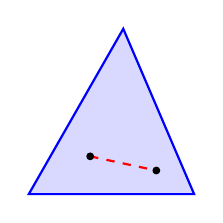
\begin{tikzpicture}[scale=0.6]
        % Fill and draw the triangle
        \filldraw[fill=blue!15, draw=blue, thick] 
            (-1.5, -1) -- (2, -1) -- (0.5, 2.5) -- cycle;
        
        % Points and line segment showing convexity
        \coordinate (A) at (-0.2, -0.2);
        \coordinate (B) at (1.2, -0.5);
        \draw[thick, red, dashed] (A) -- (B);
        \filldraw[black] (A) circle (2pt);
        \filldraw[black] (B) circle (2pt);
    \end{tikzpicture}
    
    %\vspace{0.5cm}
    %\textbf{Triangle}\\
    %(Common Convex Set)
\end{minipage}\hfill
% Ellipse
\begin{minipage}{0.31\textwidth}
    \centering
    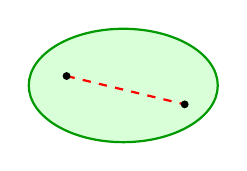
\begin{tikzpicture}[scale=0.6]
        % Fill and draw the ellipse
        \filldraw[fill=green!15, draw=green!60!black, thick] 
            (0, 0.5) ellipse (2 and 1.2);
        
        % Points and line segment showing convexity
        \coordinate (C) at (-1.2, 0.7);
        \coordinate (D) at (1.3, 0.1);
        \draw[thick, red, dashed] (C) -- (D);
        \filldraw[black] (C) circle (2pt);
        \filldraw[black] (D) circle (2pt);
    \end{tikzpicture}
    
    %\vspace{0.5cm}
    %\textbf{Ellipse}\\
    %(Common Convex Set)
\end{minipage}\hfill
% Arbitrary Convex Shape
\begin{minipage}{0.31\textwidth}
    \centering
    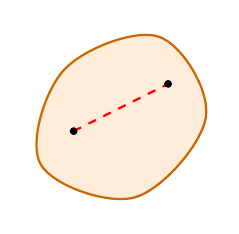
\begin{tikzpicture}[scale=0.6]
        % Fill and draw an arbitrary smooth convex polygon
        \filldraw[fill=orange!15, draw=orange!80!black, thick] 
            plot[smooth cycle, tension=0.6] coordinates 
            {(-1.5, -0.5) (0.5, -1.2) (2, 0.5) (1, 2.2) (-1, 1.5)};
        
        % Points and line segment showing convexity
        \coordinate (E) at (-0.8, 0.2);
        \coordinate (F) at (1.2, 1.2);
        \draw[thick, red, dashed] (E) -- (F);
        \filldraw[black] (E) circle (2pt);
        \filldraw[black] (F) circle (2pt);
    \end{tikzpicture}
    
    %\vspace{0.5cm}
    %\textbf{Arbitrary Shape}\\
    %(Custom Convex Set)
\end{minipage}

\vspace{1em}

\begin{definition}[Epigraph]
    \begin{shaded*}
        Let $I\subset\R$ be an interval and let $f:I\to\R$ be a function. The \textit{epigraph} of $f$ is the subset of $\R^2$ defined by
        \[\mathrm{epi}(f)\coloneqq \{(x,y)\in I\times \R : y \ge f(x)\}\subset \R^2.\]
    \end{shaded*}
\end{definition}
The following is a \textit{geometric} definition of convex functions.
\begin{definition}[Convex Function]
\label{def:epigraphconvex}
    \begin{shaded*}
        We say that a function $f:I\to\R$ is \textit{convex} if $\mathrm{epi}(f)$ is a convex set in $\R^2$.
    \end{shaded*}
\end{definition}

Intuitively, the region above the graph has no ``dents''. Unwinding this definition yields two concrete inequalities which are often easier to use in practice.

\section{Jensen's Inequality}

\begin{theorem}[Jensen's Inequality for Convex Functions]
\label{thm:jensen}
    \begin{shaded*}
        Let $I \subset \R$ be an interval. A function $f: I \to \R$ is \textit{convex} on $I$ if and only if for all $a< b \in I$, and for all $t \in [0,1]$,
        \[ f((1-t)a + tb) \le (1-t)f(a) + tf(b). \]
    \end{shaded*}
\end{theorem}
\begin{proof}
    First, assume $f:I\to\R$ satisfies the epigraph definition of convexity (Definition \ref{def:epigraphconvex}). Let $a<b$ in $I$ be arbitrary, and consider the points $x=(a,f(a))\in \mathrm{epi}(f)$ and $y=(b,f(b))\in \mathrm{epi}(f)$. By convexity of $\mathrm{epi}(f)$, using Definition \ref{def:convexset} for convex sets, we see that the line segment between $x$ and $y$ lies in $\mathrm{epi}(f)$, but for $t\in[0,1]$ we have
    \[(1-t)x+ty=((1-t)a+tb, (1-t)f(a)+tf(b)),\]
    so the y-coordinate in the above point on the line segment must lie above the graph $f$ at $x=(1-t)a+tb$. In other words, we have
    \[f((1-t)a+tb)\le (1-t)f(a)+tf(b),\]
    which proves the ($\Rightarrow$) direction.

    Conversely, assume Jensen's inequality for convex functions; we wish to show that $f$ satisfies the epigraph definition of convexity, Definition \ref{def:epigraphconvex}, i.e. we need to show that $\mathrm{epi}(f)$ is a convex set in $\R^2$. Let $x,y\in \mathrm{epi}(f)$ be arbitrary, and write $x=(x_1,y_1)$, $y=(x_2,y_2)$, so $y_1\ge f(x_1)$ and $y_2\ge f(x_2)$. Therefore, for $t\in[0,1]$ we have
    \[(1-t)y_1+ty_2\ge (1-t)f(x_1)+tf(x_2)\ge f((1-t)x_1+tx_2),\]
    where the last inequality is by Jensen's inequality. This implies that
    \[(1-t)x+ty\in\mathrm{epi}(f),\]
    which finishes the proof.\qedhere
\end{proof}

The above theorem is an if and only if statement, so can be taken as an equivalent definition of a convex function. Jensen's inequality for convex functions simply states that the graph of the function always lies \textit{below} the chord connecting any two points on the graph.  



\begin{remark}
    One can think of a convex function as being shaped like a bowl; consider a convex function defined on $[0,\infty)$: it is fundamentally trying to bending upwards, though it doesn't have to. It is either trying to bend upwards for all $x>0$, but fails, in which case it is a decreasing function for $x>0$, or does eventually start pointing upwards, and continues in this way, as visualised above in the examples. Or it simply starts off as increasing, and must continue in this way to remain convex (in fact, we will see later that the slope itself must be increasing too, for a differentiable convex function).
\end{remark}

Some examples of convex functions are illustrated below. As seen in Theorem \ref{thm:jensen}, Jensen's inequality for convex functions is equivalent to our epigraph definition and simply states that the graph of the function sits below the chord drawn between any two points on the graph.

\begin{center}
\begin{minipage}{0.31\textwidth}
    \centering
    \resizebox{\linewidth}{!}{%
    \begin{tikzpicture}
        % Axes
        \draw[->] (-2.2,0) -- (2.2,0) node[right] {$x$};
        \draw[->] (0,-0.5) -- (0,3.5) node[above] {$f(x)$};
        
        % Function Curve
        \draw[thick, black, domain=-1.7:1.7, samples=50] plot (\x, {\x*\x});
        
        % Secant line showing convexity
        \draw[thick, red, dashed] (-1.2, 1.44) -- (1.4, 1.96);
        \filldraw[black] (-1.2, 1.44) circle (2pt);
        \filldraw[black] (1.4, 1.96) circle (2pt);
    \end{tikzpicture}%
    }
    
\end{minipage}\hfill
% ---------- Second Function: Absolute Value ----------
\begin{minipage}{0.31\textwidth}
    \centering
    \resizebox{\linewidth}{!}{%
    \begin{tikzpicture}
        % Axes
        \draw[->] (-2.2,0) -- (2.2,0) node[right] {$x$};
        \draw[->] (0,-0.5) -- (0,3.5) node[above] {$f(x)$};
        
        % Function Curve
        \draw[thick, black] (-1.7, 1.7) -- (0,0) -- (1.7, 1.7);
        
        % Secant line showing convexity
        \draw[thick, red, dashed] (-1.4, 1.4) -- (0.8, 0.8);
        \filldraw[black] (-1.4, 1.4) circle (2pt);
        \filldraw[black] (0.8, 0.8) circle (2pt);
    \end{tikzpicture}%
    }
\end{minipage}\hfill
% ---------- Third Function: Arbitrary Asymmetric ----------
\begin{minipage}{0.31\textwidth}
    \centering
    \resizebox{\linewidth}{!}{%
    \begin{tikzpicture}
        % Axes
        \draw[->] (-2.2,0) -- (2.2,0) node[right] {$x$};
        \draw[->] (0,-0.5) -- (0,3.5) node[above] {$f(x)$};
        
        % Function Curve (y = 0.1x^4 + 0.3x^2 - 0.4x + 0.5)
        \draw[thick, black, domain=-1.6:1.9, samples=50] 
            plot (\x, {0.1*(\x*\x*\x*\x) + 0.3*(\x*\x) - 0.4*\x + 0.5});
        
        % Secant line showing convexity
        \draw[thick, red, dashed] (-1, 1.3) -- (1.5, 1.075);
        \filldraw[black] (-1, 1.3) circle (2pt);
        \filldraw[black] (1.5, 1.075) circle (2pt);
    \end{tikzpicture}%
    }
\end{minipage}
\end{center}



\begin{definition}[Strictly Convex Function]
    \begin{shaded*}
        A function $f: I \to \R$ is \textit{strictly convex} on $I$ if, for all $a<b \in I$, and for all $t \in (0,1)$:
        \[ f((1-t)a + tb) < (1-t)f(a) + tf(b). \]
    \end{shaded*}
\end{definition}
\begin{remark}
    Strict convexity is a stronger property for a function $f:I\to\R$ to satisfy, and through it we see the relevance of our study of convexity: convexity is related to minimisation problems. Intuitively you can see that if a strictly convex function is differentiable, and if it has a critical point in some place, then it is unique and it is a global minimiser, because once the function starts bending upwards, it must keep increasing if it is convex everywhere (we will see this later).
\end{remark}

It is often convenient to have an explicit function defined on $I$, rather than a parameterisation, when working with Jensen's inequality and chords:

\begin{definition}[Chord line]
\label{def:chordline}
    \begin{shaded*}
        Let $f:I\to\R$ be a function and let $a<b$ in $I$. We denote by $\ell_{a,b}:\R\to\R$ the affine function whose graph is the straight line through $(a,f(a))$ and $(b,f(b))$:
        \[\ell_{a,b}(x)=\frac{f(b)-f(a)}{b-a}(x-a)+f(a).\]
    \end{shaded*}
\end{definition}

\begin{lemma}
    \begin{shaded*}
        Let $f:I\to\R$ be a function. The following are equivalent:
        \begin{enumerate}
            \item[1.] $f$ is convex on $I$
            \item[2.] For all $a<b$ in $I$ and for all $x\in[a,b]$, \[f(x)\le \ell_{a,b}(x).\]
        \end{enumerate}
    \end{shaded*}
\end{lemma}
\begin{proof}
    Exercise.\qedhere
\end{proof}

\section{Slope Monotonicity}

While the graph of a convex function lies \textit{below} (or on) the chord inside the interval $[a,b]$, the \textit{opposite} is true outside the interval; the graph lies above the extension of the same chord. Draw a few pictures to convince yourself of this.

\begin{lemma}[Chord Extension Inequality]
\label{lem:chordextension}
    \begin{shaded*}
        Let $f: I \to \R$ be convex. For any $a, b \in I$ with $a < b$, let $\ell_{a,b}(x)$ be the line passing through $(a, f(a))$ and $(b, f(b))$. Then for all $x \in I \setminus [a,b]$, the graph lies above the chord:
        $$ f(x) \ge \ell_{a,b}(x) $$
    \end{shaded*}
\end{lemma}

\begin{proof}
    Suppose $x > b$. Since $a < b < x$, the point $b$ lies strictly between $a$ and $x$. Therefore, we can express $b$ as a convex combination of $a$ and $x$. For some $t\in\R$, we have
\[ b = (1-t)a + tx. \]

Solving for $t$, we get $t = \frac{b-a}{x-a}$. Because $b$ is strictly between $a$ and $x$, we know $t \in (0, 1)$.

Applying Jensen's inequality on the chord from $a$ to $x$, we get
\[ f(b) \le (1-t)f(a) + t f(x). \]

Isolating $f(x)$ yields
\begin{align*}
t f(x) &\ge f(b) - (1-t)f(a) \\
f(x) &\ge \frac{1}{t}f(b) - \frac{1-t}{t}f(a)
\end{align*}

By using our definition of $t$, we get
\[ f(x) \ge \frac{x-a}{b-a}f(b) - \frac{x-b}{b-a}f(a) \quad (\dagger) \]

To finish, we verify this matches the equation of the secant line $\ell_{a,b}(x)$. The standard point-slope form for the line through $a$ and $b$ from Definition \ref{def:chordline} is:
\[ \ell_{a,b}(x) = \frac{f(b)-f(a)}{b-a}(x-a) + f(a), \]

and rearranging we have
\begin{align*}
\ell_{a,b}(x) &= f(a)\left(1 - \frac{x-a}{b-a}\right) + f(b)\left(\frac{x-a}{b-a}\right) \\
&= f(a)\left(\frac{b-a - x + a}{b-a}\right) + f(b)\left(\frac{x-a}{b-a}\right) \\
&= -f(a)\left(\frac{x-b}{b-a}\right) + f(b)\left(\frac{x-a}{b-a}\right),
\end{align*}

which matches the inequality $(\dagger)$. Hence we have
\[ f(x) \ge \ell_{a,b}(x), \]
which completes the proof.\qedhere
\end{proof}



\begin{lemma}[Slope Monotonicity Lemma]
\label{lem:slopemon}
    \begin{shaded*}
        Let $f: I \to \R$ be a convex function. Then for any $a < b < c$ in $I$, the slopes of the chords are monotonically increasing:
        \[ \frac{f(b)-f(a)}{b-a} \le \frac{f(c)-f(b)}{c-b}. \]
        If $f$ is strictly convex, these inequalities are strict.
    \end{shaded*}
\end{lemma}

\begin{proof}
    Note that for every $x \in [b, c]$ we have
\[ \ell_{a,b}(x) \le f(x) \le \ell_{b,c}(x). \]
Indeed, the inequality $\ell_{a,b}(x) \le f(x)$ holds because $x \ge b$ lies outside $[a, b]$, so we can apply the chord extension inequality to the chord through $(a, f(a))$ and $(b, f(b))$. The inequality $f(x) \le \ell_{b,c}(x)$ holds by convexity on $[b, c]$.
Therefore, for all $x \in [b, c]$,
\[ \ell_{a,b}(x) \le \ell_{b,c}(x). \]
We now write both lines in terms of $x - b$ (this makes the comparison transparent):
\[ \ell_{a,b}(x) = \frac{f(b) - f(a)}{b - a}(x - b) + f(b), \qquad \ell_{b,c}(x) = \frac{f(c) - f(b)}{c - b}(x - b) + f(b). \]
Since $\ell_{a,b}(x) \le \ell_{b,c}(x)$ for all $x \in [b, c]$ and $x - b \ge 0$ on this interval (with $x - b > 0$ as soon as $x > b$), we conclude that the coefficient of $(x - b)$ on the left is at most the coefficient on the right, namely
\[ \frac{f(b) - f(a)}{b - a} \le \frac{f(c) - f(b)}{c - b}. \]
This completes the proof. \qedhere
\end{proof}

\begin{corollary}
\label{cor:threechord}
    \begin{shaded*}
        Let $f:I\to\R$ be convex. Then for any $a<b<c<d$ in $I$, we have
        \[\frac{f(b)-f(a)}{b-a}\le \frac{f(d)-f(c)}{d-c}.\] 
    \end{shaded*}
\end{corollary}
\begin{proof}
    Apply Lemma \ref{lem:slopemon} to $a<b<c$ and then to $b<c<d$:
\[ \frac{f(b) - f(a)}{b - a} \le \frac{f(c) - f(b)}{c - b} \le \frac{f(d) - f(c)}{d - c}. \]\qedhere
\end{proof}

\begin{theorem}
    \begin{shaded*}
        Let $I\subset\R$ be an open interval, and let $f:I\to\R$ be convex. If $f$ is differentiable at two points $s<t$ in $I$ then \[f'(s)\le f'(t).\]
    \end{shaded*}
\end{theorem}
\begin{proof}
    Fix $s<\alpha<t$ and $t<\beta$ such that $\alpha,\beta\in I$. By Corollary \ref{cor:threechord}, we have
    \[\frac{f(\alpha)-f(s)}{\alpha -s}\le \frac{f(\beta)-f(t)}{\beta - t}.\]
    Treating $\beta$ as fixed, and taking the limit as $\alpha \to s^+$ in the above inequality, and using the differentiability of $f$ at $s$, we get
    \[f'(s)\le \frac{f(\beta) - f(t)}{\beta - t},\]
    and letting $\beta\to t^+$ in the above inequality, and using the differentiability of $f$ at $t$ yields $f'(s)\le f'(t)$, which completes the proof.\qedhere
\end{proof}

\begin{corollary}[Monotonicity of the Derivative]
    \begin{shaded*}
        Let $f$ be differentiable on an open interval $I$. Then $f$ is convex on $I$ if and only if its derivative $f'$ is increasing on $I$. Furthermore, $f$ is strictly convex on $I$ if and only if $f'$ is strictly increasing on $I$.
    \end{shaded*}
\end{corollary}

\begin{remark}[The Second Derivative and Strict Convexity]
    If $f$ is twice-differentiable, $f$ being convex is equivalent to $f''(x) \ge 0$ for all $x \in I$. 
    However, if $f$ is \textit{strictly} convex, it is a false statement that $f''(x) > 0$ everywhere. The standard counterexample is $f(x) = x^4$. It is strictly convex everywhere, yet $f''(0) = 0$. 
\end{remark}

\section{Regularity of Convex Functions}

\begin{theorem}[Continuity of Convex Functions]
\label{thm:convexcontinuity}
    \begin{shaded*}
        Let $I\subset\R$ be an open interval. If $f: I \to \R$ is convex on $I$, then $f$ is continuous on $I$.
    \end{shaded*}
\end{theorem}
\begin{proof}
    Let $a\in I$ be arbitrary; we wish to show that $f$ is continuous at $a$. First, since $I$ is an open interval we can let $\delta>0$ be such that $[a-\delta,a+\delta]\subset I$. Fix $t\in (a-\delta,a)$. By convexity of $f$ on $[a-\delta,a]$, we have
    \[f(t)\le \ell_{a-\delta,a}(t).\]
    By the Chord Extension Inequality (Lemma \ref{lem:chordextension}) on $[a,a+\delta]$, we also have
    \[\ell_{a,a+\delta}(t)\le f(t).\]Therefore, for all $x\in(a-\delta,a)$, we have \[\ell_{a,a+\delta}(x)\le f(x)\le \ell_{a-\delta,a}(x).\]
    Both chord lines are continuous and by construction satisfy $\ell_{a-\delta,a}(a)=\ell_{a,a+\delta}(a)=f(a)$, so by the squeeze theorem for limits of functions,
    \[\lim_{x\to a^-}f(x)=f(a).\]
    For the right limit, the argument is identical; indeed, using the same argument as above, for every $x\in(a,a+\delta)$ we have \[\ell_{a-\delta,a}(x)\le f(x)\le \ell_{a,a+\delta}(x),\]
    and letting $x\to a^+$ in the above inequality and using the continuity of the chord lines yields $\lim_{x\to a^+}f(x)=f(a)$, so $f$ is continuous at $a$.\qedhere
\end{proof}

The proof of the above theorem is key: near an interior point $a$, convexity traps the graph between two straight lines that meet at $(a,f(a))$.

An important subtlety of the proof is that the hypothesis of $a$ being interior was crucial so that we could extend the chords.
Because of that the argument does not work at the end points.
Indeed, as the next example shows, the result is not true at the boundary of an interval.

\begin{example}
    The requirement that $I$ be an \textit{open} interval is strictly necessary. A function can be convex on a closed interval but discontinuous at the boundary. For example, consider $f: [0,1] \to \R$ defined by $f(x) = 0$ for $x \in (0,1)$ and $f(0)=1, f(1)=1$. This function satisfies the convexity inequality everywhere on $[0,1]$ but is clearly discontinuous at the endpoints. Thus, for a general interval $I$, we can only guarantee that $f$ is continuous on the \textit{interior} of $I$.
\end{example}

\begin{remark}
    Convexity only implies continuity (on open intervals); it does not imply differentiability. The classic counterexample is $f(x) = |x|$, which is strictly convex on $\R$ but not differentiable at $x=0$.
\end{remark}

When a convex function \textit{is} differentiable, its local geometry becomes highly constrained:

\begin{theorem}[Tangent Line Characterisation]
\label{thm:convextangent}
    \begin{shaded*}
        If $f: I \to \R$ is convex and differentiable at an interior point $x_0 \in I$, then the graph of $f$ sits globally above its tangent line at $x_0$:
        $$ f(x) \ge f(x_0) + f'(x_0)(x-x_0) \quad \text{for all } x \in I $$
    \end{shaded*}
\end{theorem}

\begin{proof}
    Let $x > x_0$. By the Slope Monotonicity Lemma, for any fixed $t \in (x_0, x)$, the slopes of the chords satisfy:
    \[ \frac{f(t)-f(x_0)}{t-x_0} \le \frac{f(x)-f(x_0)}{x-x_0} \]
    Taking the limit as $t \to x_0^+$ (which exists because $f$ is differentiable at $x_0$), we get
    \[f'(x_0) \le \frac{f(x)-f(x_0)}{x-x_0}, \]
    since limits preserve non-strict inequalities.
    Multiplying by $(x-x_0) > 0$ and rearranging yields $f(x) \ge f(x_0) + f'(x_0)(x-x_0)$. The argument for $x < x_0$ is symmetric.\qedhere
\end{proof}

\begin{remark}
    So convexity can be rephrased as: every tangent line (where it exists) is a global under-estimate for the function. Intuitively, it can be seen as a ``supporting line'' on which the function sits.
\end{remark}

\subsection{Minimisation}

Convexity provides incredibly strong guarantees about optimisation and bounds.

\begin{theorem}[Uniqueness of Critical Points]
    \begin{shaded*}
        Let $f: I \to \R$ be strictly convex and differentiable on an open interval $I$. Then $f$ has at most one critical point on $I$. Moreover, if $f'(c) = 0$ for some $c \in I$, then $c$ is the unique global minimiser of $f$ on $I$.
    \end{shaded*}
\end{theorem}

\begin{proof}
    Suppose $f'(c) = 0$. By Theorem \ref{thm:convextangent}, we have
    \[ f(x) \ge f(c) + f'(c)(x-c) = f(c) + 0 = f(c) \]
    Because $f$ is strictly convex, this inequality is strict for $x \neq c$, making $c$ the unique global minimum. 
    Furthermore, because $f$ is strictly convex, $f'$ is strictly increasing. A strictly increasing function can intersect the axis $f'(x) = 0$ at most once, meaning there can be at most one critical point.
\end{proof}



\begin{theorem}
    \begin{shaded*}
        Let $I\subset\R$ be a bounded interval and let $f:I\to\R$ be a convex function. Then $f$ is bounded below.
    \end{shaded*}
\end{theorem}

\begin{proof}
    Fix two points $s, t$ in the interior of $I$ such that $s < t$. We can partition the interval $I$ into the closed sub-interval $[s, t]$ and the remaining outside portion $I \setminus [s, t]$.

First, consider the interval $[s, t]$. Since $f$ is convex, by Theorem \ref{thm:convexcontinuity}, $f$ is continuous on the interior of $I$. Since $s$ and $t$ are in the interior of $I$, the closed interval $[s, t]$ lies entirely within the interior of $I$. Therefore, $f$ is continuous on $[s, t]$. By the Extreme Value Theorem (Theorem \ref{thm:evt}), $f$ attains a minimum on this closed, bounded interval. Thus, there exists some $M_1 \in \mathbb{R}$ such that:
\[ f(x) \ge M_1 \quad \text{for all } x \in [s, t]. \]

Next, consider the region outside this sub-interval, $I \setminus [s, t]$. Let $\ell_{s,t}(x)$ be the secant line passing through the points $(s, f(s))$ and $(t, f(t))$. By the Chord Extension Inequality (Lemma \ref{lem:chordextension}), the graph of a convex function lies above its extended secant chords outside the interval $[s,t]$. Therefore:
\[ f(x) \ge \ell_{s,t}(x) \quad \text{for all } x \in I \setminus [s, t]. \]
Since $I$ is a bounded interval, $x$ cannot approach $\pm\infty$. The secant line $\ell_{s,t}(x)$ is a linear function, and any linear function restricted to a bounded domain is bounded below. Thus, there exists some $M_2 \in \mathbb{R}$ such that $\ell_{s,t}(x) \ge M_2$ for all $x \in I$. This implies:
\[ f(x) \ge M_2 \quad \text{for all } x \in I \setminus [s, t]. \]

Finally, let $M = \min\{M_1, M_2\}$. It follows that $f(x) \ge M$ for all $x \in I$. Therefore, $f$ is bounded below on $I$.\qedhere
\end{proof}

\begin{exercise*}
    Let $f:[0,\infty)\to\R$ be convex and bounded. Show that $\lim_{x\to\infty}f(x)$ exists and is finite.
\end{exercise*}

\begin{exercise*}
    In the setting of the above exercise, assume in addition that $f$ is differentiable on $(0,\infty)$. Prove that $\lim_{x\to\infty}f'(x)=0$.
\end{exercise*}




\end{document}